%\documentclass[conference,a4paper,10pt,oneside,final]{tp}
\documentclass[10pt]{book}
\usepackage[utf8]{inputenc}   						% caracteres especiales (acentos, eñes)
\usepackage{mylatex} % mi paquete de características LaTeX

  
%------------------------------------------------------------------------------------------------------------------------------------------
%	ENCABEZADO Y PIE DE PÁGINA
%------------------------------------------------------------------------------------------------------------------------------------------
\pagestyle{fancy}
\fancyhf{}
\lhead{Sistemas Operativos}
\chead{Año 2016}
\rhead{Resumen}
\headsep = 1.5 cm
\lfoot{Gentile - Rosales - Santellán}
\cfoot{SO - Resumen}
\rfoot{\thepage}

%------------------------------------------------------------------------------------------------------------------------------------------
%	AJUSTES INICIALES
%------------------------------------------------------------------------------------------------------------------------------------------


%------------------------------------------------------------------------------------------------------------------------------------------
%	INICIO DEL DOCUMENTO
%------------------------------------------------------------------------------------------------------------------------------------------
\begin{document}

%------------------------------------------------------------------------------------------------------------------------------------------
%	COMIENZO DE CARÁTULA
%------------------------------------------------------------------------------------------------------------------------------------------
\begin{titlepage}
\newcommand{\HRule}{\rule{\linewidth}{0.5 mm}} % Defines a new command for the horizontal lines, change thickness here
\center % Center everything on the page

%------------------------------------------------------------------------------------------------------------------------------------------
%	SECCIÓN DE ENCABEZAMIENTO
%------------------------------------------------------------------------------------------------------------------------------------------ 
\textsc{\huge Universidad Nacional del Litoral}\\[1 cm]
\textsc{\LARGE Facultad de Ingeniería y Ciencias Hídricas}\\[0.5 cm]
\textsc{\Large Sistemas Operativos}\\[2 cm]

%------------------------------------------------------------------------------------------------------------------------------------------
%	SECCIÓN DE TÍTULO
%------------------------------------------------------------------------------------------------------------------------------------------
\HRule \\[0.8 cm]
{ \huge \bfseries Resumen}\\[0.5 cm] % Title of your document
\HRule \\[2 cm]
 
%------------------------------------------------------------------------------------------------------------------------------------------
%	SECCIÓN DE AUTOR
%------------------------------------------------------------------------------------------------------------------------------------------
\begin{minipage}{0.4\textwidth}
\begin{flushleft} \large
\emph{Autores:}\\
Mario \textsc{Rosales}\\
Franco \textsc{Santellán}\\
Carlos \textsc{Gentile}\\
\end{flushleft}
\end{minipage}
~
\begin{minipage}{0.4\textwidth}
\begin{flushright} \large
\emph{E-mail:} \\
mariorosales941@gmail.com\\
franco\_chimi@hotmail.com\\
csgentile@gmail.com\\ % Supervisor's Name
\end{flushright}
\end{minipage}\\[2 cm]

% If you don't want a supervisor, uncomment the two lines below and remove the section above
%\Large \emph{Author:}\\
%John \textsc{Smith}\\[3cm] % Your name

%------------------------------------------------------------------------------------------------------------------------------------------
%	SECCIÓN DE FECHA
%------------------------------------------------------------------------------------------------------------------------------------------
\newdateformat{monthyeardate}{\monthname[\THEMONTH], \THEYEAR}
{\large \textsc{\monthyeardate\today}}\\[5 cm] % Date, change the \today to a set date if you want to be precise

%------------------------------------------------------------------------------------------------------------------------------------------
%	SECCIÓN DE LOGO
%------------------------------------------------------------------------------------------------------------------------------------------

\includegraphics{img/logo.jpg}\\[3 cm] % Include a department/university logo - this will require the graphicx package
 
%------------------------------------------------------------------------------------------------------------------------------------------
\vfill % Fill the rest of the page with whitespace
\end{titlepage}
%------------------------------------------------------------------------------------------------------------------------------------------
%	FIN DE CARÁTULA
%------------------------------------------------------------------------------------------------------------------------------------------

%------------------------------------------------------------------------------------------------------------------------------------------
%	COMIENZO DEL DOCUMENTO PRINCIPAL
%------------------------------------------------------------------------------------------------------------------------------------------
\setcounter{chapter}{4}
\chapter{Sincronización de acceso a los objetos compartidos}
Los programas multihilo extienden el modelo tradicional, de un solo subproceso de programación de manera que cada hilo proporciona un único flujo secuencial de ejecución compuesto por instrucciones conocidas. Si un programa tiene hilos independientes que operan en subconjuntos completamente separados de la memoria, podemos razonar sobre cada hilo por separado. En este caso, el razonamiento acerca de los hilos independientes difiere poco del razonamiento acerca de una serie de programas independientes, de un único subproceso.

Sin embargo, la mayoría de los programas multihilo tienen tanto el estado para cada hilo (por ejemplo, registros de pila y un hilo) y el estado compartido (por ejemplo, variables compartidas en la pila). Los hilos de lectura y escritura cooperan con el estado compartido.

Compartir el estado es útil porque permite que los hilos se comuniquen, que coordinen el trabajo y compartan información. Por ejemplo, en el ejemplo de un GPS, una vez que un subproceso termina de descargar una imagen detallada de la red, comparte los datos de imagen con un hilo de renderizado que señala a la nueva imagen en la pantalla.

Por desgracia, cuando los hilos cooperan compartiendo sus estados, escribir programas multihilo correctos se vuelve mucho más difícil. La mayoría de los programadores están acostumbrados a pensar ''secuencialmente'' al razonar acerca de los programas. Por ejemplo, a menudo razonamos acerca de la serie de estados atravesados por un programa que ejecuta una secuencia de instrucciones. Sin embargo, este modelo secuencial de razonamiento no funciona en los programas de hilos cooperantes, por tres razones:

\begin{enumerate}
\item \textbf{La ejecución del programa depende de las posibles intercalaciones de acceso a hilos de estado compartido.} Por ejemplo, si dos hilos escriben una variable compartida, un hilo con el valor 1 y el otro con el valor 2, el valor final de la variable depende de cuál de los hilos acaba último.

Aunque este ejemplo es simple, el problema es grave porque los programas tienen que trabajar para cualquier posible intercalación. En particular, recuerdan que los programadores de hilos no deben hacer ninguna suposición sobre la velocidad relativa a la que operan sus hilos. Peor aún, como los programas crecen, hay una explosión combinatoria en el número de posibles intercalaciones.

\item \textbf{La ejecución del programa puede ser determinista.} Diferentes ejecuciones del mismo programa pueden producir resultados diferentes. Por ejemplo, el programador puede tomar diferentes decisiones de planificación, el procesador puede funcionar a una frecuencia diferente, u otro programa se ejecuta simultáneamente puede afectar a la caché de índice de aciertos. Incluso las técnicas de depuración comunes - como la ejecución de un programa con un depurador, volver a compilar con la opción -g en lugar de -O, o la adición de un printf - pueden cambiar el comportamiento de un programa.

Jim Gray, el ganador del premio ACM Turing 1998, acuñó el término \textit{Heisenbug} para los insectos que desaparecen o cambian el comportamiento cuando intenta examinarlos. La programación multihilo es una fuente común de heisenbug. Por el contrario, \textit{Bohrbugs} son deterministas y por lo general mucho más fácil de diagnosticar.

\item \textbf{Los compiladores y hardware del procesador pueden cambiar el orden de las instrucciones.} Los compiladores modernos e instrucciones de reabastecimiento de hardware mejoran el rendimiento. Esta reordenación es generalmente invisible para los programas de un solo subproceso; compiladores y procesadores de tener cuidado de asegurarse de que las dependencias dentro de una sola secuencia de instrucciones - es decir, dentro de un tema - se conservan. Sin embargo, el reordenamiento puede ser visible cuando varios subprocesos interactúan a través de acceso a variables compartidas.
\end{enumerate}

Teniendo en cuenta estos desafíos, el código multihilo puede introducir errores reproducibles sutiles, no deterministas, y no gubernamentales. En este capítulo se describe un enfoque estructurado para la sincronización del estado compartido en programas multihilo. En lugar de la dispersión de acceso a estos recursos compartidos en todo el programa e intentar razonamiento \textit{ad hoc} sobre lo que ocurre cuando se accede a los hilos se intercalan de diversas maneras, un mejor enfoque consiste en: $(1)$ la estructura del programa para facilitar el razonamiento acerca de la concurrencia, y $(2)$ utiliza un conjunto de primitivas de sincronización estándar para controlar el acceso a estos recursos compartidos. Este enfoque da un poco de libertad, pero si usted sigue constantemente las reglas que se describen en este capítulo, a continuación, el razonamiento sobre programas con estado compartido se convierte en mucho más simple.

La primera parte de este capítulo profundiza en los desafíos que enfrentan los programadores de subprocesos múltiples y el por qué es peligroso tratar de razonar acerca de todas las posibles intercalaciones de hilos en el caso general, no estructurada. El resto del capítulo describe la forma de estructurar los objetos compartidos en programas multihilo para que podamos razonar sobre ellos. En primer lugar, la estructura del Estado compartido de un programa multihilo como un conjunto de objetos compartidos que encapsulan el estado compartido, así como definir y limitar cómo se puede acceder al estado. En segundo lugar, para evitar el razonamiento \textit{ad hoc} sobre los posibles intercalamientos de acceso a las variables de estado dentro de un objeto compartido, se describe cómo los objetos compartidos pueden utilizar un pequeño conjunto de primitivas de sincronización - cerrojos y variables de condición - para coordinar el acceso a su estado por diferentes hilos. En tercer lugar, para simplificar el razonamiento sobre el código en objetos compartidos, se describe un conjunto de mejores prácticas para escribir el código que implementa cada objeto compartido. Por último, se profundiza en los detalles de cómo implementar primitivas de sincronización.

La programación multihilo tiene la reputación de ser difícil. Estamos de acuerdo en que se necesita atención, pero este capítulo proporciona un conjunto de reglas simples que cualquiera puede seguir para implementar los objetos que se pueden compartir con seguridad por varios subprocesos.

\section{Challenges - Desafíos}
Comenzamos este capítulo con el principal reto de la programación multihilo: la ejecución de un programa multihilo depende de los accesos intercalados del subproceso diferente a la memoria compartida, que pueden hacer que sea difícil para razonar acerca de depuración o de estos programas. En particular, la ejecución de hilos cooperantes puede verse afectada por las condiciones de carrera.

\subsection{Condiciones de Carrera}
Una condición de carrera se produce cuando el comportamiento de un programa depende de la intercalación de las operaciones de diferentes hilos. En efecto, los hilos corren una carrera entre sus operaciones y los resultados de la ejecución del programa depende de quién gane la carrera. Razonar sobre programas sencillos incluso con condiciones de carrera puede ser difícil. Para apreciar esto, ahora nos fijamos en tres programas multihilo muy simples.

\textbf{El programa de hilos cooperantes más simple del mundo.} Supongamos que ejecuta un programa con dos hilos que hacen lo siguiente: en el Hilo A se ejuta $x = 1$ y en el Hilo B se ejecuta $x = 2$. El resultado puede ser $x = 1$ o $x = 2$ dependiendo de qué hilo gane o pierda la carrera para setear el valor de $x$.

\textbf{El segundo programa de hilos cooperantes más pequeño del mundo.} Supongamos que en un principio $y = 12$, y se corre un programa con dos hilos que hacen lo siguiente: en el Hilo A se ejecuta $x = y + 1$ y en el Hilo B se ejecuta $y = y * 2$. El resultado es $x = 13$ si el subproceso A se ejecuta en primer lugar, o $x = 25$ si es B quien se ejecuta primero. Más precisamente, obtenemos $x = 13$ si el hilo A se lee antes de las actualizaciones del hilo B y, obtenemos $x = 25$ si las actualizaciones del hilo B se lee antes del hilo A.

\textbf{El tercer programa de hilos cooperantes mas pequeño del mundo.} Supongamos que en un principio $x = 0$ y se corre un programa con dos hilos que hacen lo siguiente: en el Hilo A se ejecuta $x = x + 1$ y en el Hilo B se ejecuta $x = x + 
$. Obviamente, un posible resultado es $x = 3$. Por ejemplo, el Hilo A se ejecuta hasta el final y luego el Hilo B se ejecuta hasta su finalización. Sin embargo, también podemos obtener $x = 2$ ó $x = 1$. En particular, cuando escribimos una sola declaración como $x = x + 1$, los compiladores de muchos procesadores producen múltiples instrucciones, tales como: $(1)$ la posición de memoria de carga de registros de $x$, $(2)$ añadir al menos $1$ de dicho registro, y $(3)$ almacenar el resultado de la posición de memoria $x$. Si desensamblamos el programa anterior en simples pseudo-ensamblaje de código, podemos ver algunas de las posibilidades.

\subsection{Operaciones Atómicas}
Cuando nos hemos desmontado el código en el último ejemplo, podríamos razonar acerca de las operaciones atómicas, operaciones indivisibles que no pueden ser intercaladas con o divididas por otras operaciones. En la mayoría de las arquitecturas modernas, una carga o almacenamiento (load o store) de una palabra de $32$ bits desde o a la memoria es una operación atómica. Por lo tanto, el análisis previo razonó sobre el intercalado de cargas y almacenamientos atómicos en la memoria.

Por el contrario, una carga o almacenamiento no es siempre una operación atómica. Dependiendo de la implementación de hardware, si dos hilos almacenan el valor de un registro de coma flotante de 64 bits a una dirección de memoria, el resultado final podría ser el primer valor, el segundo valor, o una mezcla de los dos.

\subsection{Too Much Milk - Demasiada Leche}
Aunque se podría, en principio, la razonar cuidadosamente acerca de las posibles intercalaciones de cargas y almacenamientos atómicos de diferentes hilos, hacerlo es complicado y propenso a errores. Más tarde, se presenta un mayor nivel de abstracción para la sincronización de hilos, pero primero se ilustran los problemas con el uso de las cargas y almacenamientos atómicos que utilizan un problema simple llamado, ''demasiada leche''. El ejemplo es deliberadamente sencilla; programas concurrentes del mundo real son a menudo mucho más compleja. Aun así, el ejemplo muestra la dificultad de razonar sobre el acceso a intercalada estado compartido. Los modelos de problemas de demasiada leche entre dos compañeros que comparten un refrigerador y que - como buenos compañeros - se aseguran de que el refrigerador esté siempre bien abastecido con leche.

Podemos modelar cada compañero de habitación como un hilo y el número de botellas de leche en la nevera con una variable en la memoria. Si las únicas operaciones atómicas en estado compartido son cargas y almacenamientos atómicos en la memoria, ¿hay una solución al problema de demasiada leche que garantiza tanto la seguridad (el programa nunca entra en mal estado) y la vida de la conexión (el programa entrará eventualmente en un buen estado)? Aquí, nos esforzamos por las siguientes propiedades:
\begin{itemize}
\item Safety (Seguridad): Nunca más de una persona compra la leche.
\item Liveness: Si se necesita la leche, alguien finalmente lo compra.
\end{itemize}

\textbf{Solución $1$.} La idea básica es que un compañero de habitación deje una nota en la nevera antes de ir a la tienda. La forma más sencilla de dejar esta nota - dado nuestro modelo de programación que hemos compartido memoria en el que podemos realizar cargas y amacenamiento atómicos - es fijar una bandera cuando va a comprar leche y para comprobar este indicador antes de ir a comprar leche.

Desafortunadamente, esta implementación puede violar la seguridad. Por ejemplo, el primer hilo podría ejecutar todo incluyendo la verificación del valor de la leche y luego el contexto ha cambiado. A continuación, el segundo hilo podría funcionar a través de todo este código y comprar leche. Por último, el primer hilo podría ser re-programado, ver se esa nota es cero, dejar la nota, comprar más leche, y eliminar la nota, dejando el sistema con $leche == 2$.

Esta ''solución'' empeora el problema. El código anterior por lo general funciona, pero puede fallar de vez en cuando el programador hace justo lo (mal o) lo correcto. Hemos creado una Heisenbug que hace que el programa falle ocasionalmente en formas que pueden ser muy difíciles de reproducir (por ejemplo, probablemente sólo cuando el alumno está mirando a ella o cuando el CEO está demostrando un nuevo producto en una feria comercial).

\textbf{Solución 2.} En la solución 1, el compañero de habitación comprueba la nota antes de ajustarla. Esto abre la posibilidad de que un compañero ya ha tomado la decisión de comprar la leche antes de notificar a la otro compañero de cuarto de esa decisión. Si utilizamos dos variables para las notas, un compañero puede crear una nota antes de comprobar la otra nota y tomar la decisión de comprar.

Si el primer hilo ejecuta la ruta de un código y el segundo hilo ejecuta el código, este protocolo es seguro; haciendo que cada hilo de escribir una nota (''yo podría comprar leche'') antes de decidirse a comprar leche, aseguramos la seguridad de la propiedad: a lo sumo un hilo compra leche.

Aunque esta intuición es sólida, lo que demuestra la propiedad de seguridad sin enumerar todas las posibles intercalaciones que  requieren cuidado.

\textbf{Safety Proof - Prueba de seguridad.} Supongamos por el bien de la contradicción que el algoritmo no es seguro - tanto A como B compran leche. Tenga en cuenta el estado de las dos variables (noteb, leche) cuando el hilo A está en la línea marcada A1, en el preciso momento cuando se produce la carga atómica de noteb de la memoria compartida para el registro de una. Hay tres casos a considerar:
\begin{itemize}
\item Caso 1: (noteB $= 1$, la leche = cualquier valor). Este estado contradice la suposición de que el hilo Una compra leche y llega a A3.
\item Caso 2: (noteb $= 0$, leche $> 0$). En este sencillo programa, la leche de la propiedad $> 0$ es una característica estable - una vez que se convierte en realidad, sigue siendo cierto para siempre. Por lo tanto, si la leche $> 0$ es cierto cuando A está en A1, la prueba de A en la línea A2 fallará, y A no va a comprar la leche, lo que contradice nuestra suposición.
\item Caso 3: (noteb $= 0$, leche $= 0$). Sabemos que el hilo B debe actualmente no se encuentre ejecutando cualquiera de las líneas marcadas B1-B5. También sabemos que, o bien NotaA $== 1$ o leche $> 0$ serán verdaderas de ahora en adelante (Notaa o leche es también una característica estable). Esto significa que B no puede comprar la leche en el futuro (ya sea en la prueba B1 o B2 debe fallar), lo que contradice nuestra suposición de que tanto A como B comprar leche.
\end{itemize}

Puesto que cada caso contradice la suposición, el algoritmo es seguro.

\textbf{Liveness - Vida de la conexión.} Por desgracia, la solución 2 no asegura la vida de la conexión. En particular, es posible que ambos hilos para establecer sus respectivas notas, para cada hilo para comprobar la nota del otro hilo, y por tanto de las discusiones para decidir no comprar leche. Esto nos lleva a la Solución 3.

\textbf{Solución 3.} La solución $2$ era seguro porque un hilo podría evitar la compra de leche si había alguna posibilidad de que el otro hilo podría comprar leche. Para la solución $3$, nos aseguramos de que al menos uno de los hilos determina si el otro hilo ha comprado la leche o no antes de decidir si comprar o no. En particular, hacemos lo siguiente:

Podemos demostrar que la solución $3$ es seguro usar un argumento similar al que se utilizó para la solución $2$. Para demostrar que la solución $3$ es en vivo, observar que ruta de código B no tiene bucles, por lo que finalmente el hilo B debe terminar de ejecutar el código en la lista. Con el tiempo, noteB $== 0$ se convierte en verdadera y sigue siendo cierto. Por lo tanto, el subproceso A debe finalmente llegar a la línea M y decidir si comprar la leche. Si encuentra $M == 1$, a continuación, la leche ha sido comprado. Si encuentra $M == 0$, entonces se va a comprar leche. De cualquier manera, la propiedad liveness - que, si es necesario, un poco de leche se compra - se cumple.

\subsection{Discusión}
Suponiendo que el compilador y el procesador ejecutan instrucciones en el orden del programa, la prueba anterior muestra que es posible idear una solución a demasiada leche que es a la vez Safety y Liveness usando nada más que las operaciones de carga y almacenamiento atómicas en la memoria compartida. Aunque la solución que presentamos sólo funciona para los dos compañeros, no es una generalización, llamado algoritmo de Peterson, que funciona con cualquier número fijo de $n$ hilos. Sin embargo, nuestra solución para demasiada leche (y así mismo algoritmo de Peterson) no es terriblemente satisfactorio:
\begin{itemize}
\item La solución es compleja y requiere un cuidadoso razonamiento para estar convencidos de que funciona.
\item La solución es ineficiente. En demasiada leche, mientras que el hilo A está a la espera, es una espera-ocupada que consumen recursos de la CPU. En solución generalizada de Peterson, todas las discusiones pueden n-ocupados esperar. Ls espera es especialmente problemática en los sistemas modernos con derecho preferente de subprocesos múltiples, como el hilo hilado puede estar reteniendo el procesador espera de un evento que no puede ocurrir hasta que se re-programado adelantó un poco de hilo para funcionar.
\item La solución puede fallar si el compilador o hardware reorganizan las instrucciones. Esta limitación puede abordarse mediante el uso de barreras de memoria (véase el recuadro). Adición de barreras de memoria aumentaría aún más la complejidad de la implementación del algoritmo; barreras no abordan las otras limitaciones que acabamos de mencionar.
\end{itemize}

\section{La estructura de los objetos compartidos}
\begin{figure}[tbhp]
\centerline{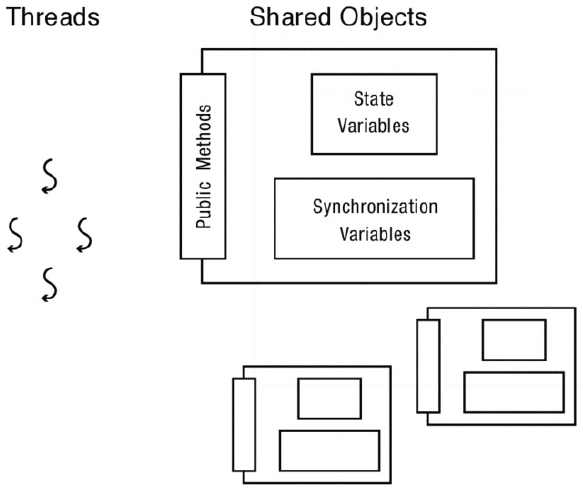
\includegraphics[scale=0.45]{img/fig0501}}
\caption{En un programa multi-hilo, hilos están separados y operan simultáneamente en objetos compartidos. Los objetos compartidos contienen ambas variables de estado y sincronización compartidos, que se utilizan para controlar el acceso concurrente a estado compartido.}
\label{fig0501}
\end{figure}

Décadas de trabajo han desarrollado un enfoque mucho más simple para escribir programas multihilo que el uso de cargas y almacenamientos atómicos. Este enfoque se extiende de la modularidad de la programación orientada a objetos para programas multihilo. Como ilustra la \textit{fig.} \ref{fig0501}, un programa multi-hilo se construye a partir de los objetos compartidos y un conjunto de hilos que operan en ellos.

Los objetos compartidos son objetos que se pueden acceder de manera segura por varios subprocesos. Todos estos recursos compartidos en un programa - incluyendo variables asignados en el montón (por ejemplo, objetos asignados con malloc o nuevo) y, variables globales estáticos - debe ser encapsulado en uno o más objetos compartidos.

Programar con objetos compartidos se extiende la programación tradicional orientado a objetos, en la cual los objetos ocultar sus detalles de implementación detrás de una interfaz limpia. De la misma manera, los objetos compartidos ocultar los detalles de la sincronización de las acciones de múltiples hilos detrás de una interfaz limpia. Los hilos que utilizan objetos compartidos sólo necesitan entender la interfaz; ellos no necesitan saber cómo el objeto compartido maneja internamente la sincronización.

Al igual que los objetos normales, los programadores pueden diseñar objetos compartidos para cualesquiera módulos, interfaces y semántica que necesita la aplicación. Cada clase de objeto compartido define un conjunto de métodos públicos en whichthreads operar. Para ensamblar el programa general de estos objetos compartidos, cada hilo se ejecuta un "bucle principal", escrita en términos de acciones sobre los métodos públicos de objetos compartidos.

Dado que los objetos compartidos encapsulan estado compartido del programa, el código de bucle principal que define medidas de alto nivel de un hilo no necesita preocuparse por los detalles de sincronización. Así, el modelo de programación se ve muy similar a la del código de un solo subproceso.

\subsection{La implementación de objetos compartidos}
Por supuesto, a nivel interno los objetos compartidos deben manejar los detalles de sincronización. Los objetos compartidos se aplican en capas.
\begin{itemize}
\item \textbf{Capa de objeto compartido.} Al igual que en la programación orientada a objetos estándar, los objetos compartidos definen la lógica específica de la aplicación y ocultan detalles internos de implementación. Externamente, parecen tener la misma interfaz que debe definir para un programa de un solo subproceso.

\item \textbf{Capa de sincronización de variable.} En lugar de la aplicación de los objetos compartidos directamente con
intercalado cuidadoso de las cargas y almacenamientos atómicos, los objetos compartidos incluyen variables de sincronización como variables miembro. las variables de sincronización, almacenados en la memoria al igual que cualquier otro objeto, pueden incluirse en cualquier estructura de datos.

Una variable de sincronización es una estructura de datos utilizada para coordinar el acceso simultáneo a estado compartido. Tanto la interfaz y la implementación de las variables de sincronización deben ser cuidadosamente diseñadas. En particular, podemos construir objetos compartidos utilizando dos tipos de variables de sincronización: Bloqueos (\textit{locks}) y Variables de Condición (\textit{condition variables}).

Las variables de sincronización coordinan el acceso a las variables de estado, que son sólo las variables miembros normales de un objeto que está familiarizado con la programación a partir de un único subproceso (por ejemplo, enteros, cadenas, arrays y punteros).

El uso de variables de sincronización simplifica la implementación de objetos compartidos. De hecho, no sólo los objetos compartidos se parecen externamente objetos de un único subproceso tradicionales, pero, mediante la aplicación, las variables de sincronización, sus implementaciones internas son bastante similares a los de los programas de un solo subproceso.

\item \textbf{La capa de instrucción Atómica.} A pesar de que las capas superiores se benefician de un modelo de programación más simple, no es tortugas hasta el final abajo. Internamente, las variables de sincronización deben gestionar los interleavings de acciones diferentes hilos.

En lugar de implementar las variables de sincronización, tales como cerrojos y variables de condición, utilizando cargas atómicas y tiendas como hemos tratado de hacer por el problema demasiada leche, las implementaciones modernas construyen las variables de sincronización utilizando instrucciones de lectura-modificación-escritura atómicas. Estas instrucciones específicos del procesador dejar un hilo tiene acceso de forma temporal y exclusiva atómica a una ubicación de memoria mientras se ejecuta la instrucción. Típicamente, la instrucción atómicamente lee una posición de memoria, hace alguna operación aritmética simple para el valor, y almacena el resultado. El hardware garantiza que las instrucciones de cualquier otro hilo con el acceso a misma posición de memoria se producen ya sea por completo antes de, o en su totalidad después de, la instrucción de lectura-modificación-escritura atómica.
\end{itemize}

\subsection{Alcance y Hoja de Ruta}
Los programas concurrentes se construyen en la parte superior de los objetos compartidos. El resto de este capítulo se centra en las capas medias de la figura - Cómo crear objetos compartidos utilizando objetos de sincronización y cómo construir objetos de sincronización de las órdenes de lectura-modificación-escritura atómicas. El capítulo 6 discute los problemas que surgen cuando se componen de varios objetos compartidos en un programa más amplio.

\section{Locks (Bloqueos): Exclusión Mutua}
Un bloqueo es una variable de sincronización que proporciona la exclusión mutua - cuando un hilo mantiene un bloqueo, ningún otro hilo puede mantenerlo (es decir, otros hilos están excluidos). Un programa tiene asociado cada cerrojo con algún subconjunto de estado compartido y requiere un hilo para mantener el bloqueo al acceder a ese estado. Entonces, sólo un hilo puede acceder al estado compartido a la vez.

La exclusión mutua simplifica en gran medida el razonamiento acerca de los programas ya que un subproceso puede realizar un conjunto arbitrario de operaciones, mientras que mantiene un bloqueo, y esas operaciones parecen ser atómicas a otros hilos. En particular, debido a que un bloqueo hace cumplir la exclusión mutua y los hilos deben sostener el bloqueo para acceder a estos recursos compartidos, ningún otro hilo puede observar un estado intermedio. Otros procesos únicamente pueden observar el estado de la izquierda después de la liberación del bloqueo.

\textbf{Bloqueo para agrupar varias operaciones.} Consideremos, por ejemplo, un objeto de cuenta de banco que incluye una lista de transacciones y un balance total. Para añadir una nueva transacción, adquirimos el bloqueo de la cuenta, añadir la nueva transacción a la lista, leer el antiguo equilibrio, modificarlo, escribir el nuevo equilibrio, y liberar el bloqueo. Para consultar el saldo y relación de las transacciones recientes, adquirimos bloqueo de la cuenta, leemos las transacciones recientes de la lista, lee el equilibrio, y liberar el bloqueo. El uso de cerrojos de esta manera garantiza que una actualización o una consulta completa antes de que comience la siguiente. Cada consulta siempre refleja el conjunto completo de transacciones recientes.

Otro ejemplo de agrupación es cuando la impresión de salida. Sin bloquear, si dos hilos llamados printf al mismo tiempo, los caracteres individuales de los dos mensajes podrían ser intercalados, garbling su significado. En cambio, en los sistemas operativos modernos multi-hilo, printf utiliza un cerrojo para asegurar que el grupo de caracteres en cada mensaje es impreso como una unidad.

Es mucho más fácil de razonar acerca de intercalación de grupos atómicos de operaciones en lugar de intercalar las operaciones individuales para dos razones. En primer lugar, hay un menor número (obviamente) interleavings a considerar. Razonar sobre interleavings sobre una base de grano más grueso reduce el número total de casos a considerar. En segundo lugar, y más importante, que podemos hacer cada grupo atómico de las operaciones corresponden a la estructura lógica del programa, lo que nos permite razonar sobre no invariantes interleavings específicos.

En particular, los objetos compartidos por lo general tienen un cerrojo que guarda todos estado de un objeto. Cada método público adquiere el bloqueo a la entrada y libera el bloqueo en la salida. Por lo tanto, el razonamiento sobre el código de una clase compartida es similar a razonar sobre el código de una clase tradicional: se asume un conjunto de invariantes cuando se llama a un método público y restablecer esas invariantes ante un público devuelve el método. Si definimos así nuestros invariantes, podemos razonar acerca de cada método de forma independiente.

\subsection{Cerrojos: API y Propiedades}
Un cerrojo permite la exclusión mutua, proporcionando dos métodos: Lock::adquieren() y Lock::Release(). Estos métodos se definen como sigue:
\begin{itemize}
\item Un bloqueo puede estar en uno de dos estados: ocupado o libre.
\item Un bloqueo se encuentra inicialmente en el estado libre.
\item Lock::adquirir espera hasta que el bloqueo es libre y luego atómicamente hace que el bloqueo OCUPADO. Comprobación del estado para ver si está libre y el establecimiento del estado de OCUPADO están juntos una operación atómica. Incluso si varios subprocesos intentan adquirir el bloqueo, a lo sumo un hilo tendrá éxito. Un hilo observa que el bloqueo es gratis y lo establece en OCUPADO; los otros hilos acaba de ver que el1 cerrojo está ocupado y esperan.
\item Lock::Bloquear la liberación hace que el bloqueo GRATIS. Si hay operaciones pendientes adquirir, este cambio de estado hace que uno de ellos para proceder.
\end{itemize}

Se describe cómo implementar los cerrojos con estas características en la sección 5.7. El uso de bloqueos hace que la solución del problema de la leche demasiado trivial. Ambos hilos corren el siguiente código:


\subsection{Semáforos}
Los \textbf{semáforos} fueron introducidos por Dijkstra en 1965 para proveer de sincronización dentro del sistema operativo. Entre los avances introducidos en el diseño de sistemas operativos se puede mencionar las formas estructuradas de utilización de la concurrencia.

Lo semáforos se definen como sigue:
\begin{itemize}
\item Un semáforo tiene un valor entero no negativo ($\geq 0$).
\item Cuando un semáforo es creado, su valor puede ser inicializado en cualquier valor entero no negativo.
\item {\mf Semaphore::P()} espera hasta que el valor sea positivo. Luego, decrementa su valor de manera atómica en 1 y retorna.
\item {\mf Semaphore::V()} incrementa de manera atómica el valor en 1. Si algún hilo se encuentra esperando en {\mf P}, entonces uno es habilitado, de forma que la llamada a {\mf P} puede decrementar exitosamente el valor y retornar.
\item No se permiten otras operaciones en un semáforo. En particular, ningún hilo puede leer directamente el valor del semáforo.
\end{itemize}

Las acciones de comprobar el valor y modificarlo se realizan en conjunto como una sola acción atómica indivisible. Se garantiza que, una vez que empieza una operación de semáforo, ningún otro proceso podrá acceder al semáforo sino hasta que la operación se haya completado o bloqueado. Esta atomicidad es absolutamente esencial para resolver problemas de sincronización y evitar condiciones de carrera.

La operación {\mf V} incrementa el valor del semáforo direccionado. Si uno o más procesos estaban inactivos en ese semáforo, sin poder completar una operación {\mf P} anterior, el sistema selecciona uno de ellos (al azar) y permite que complete su operación {\mf P} . Así, después de una
operación {\mf V} en un semáforo que contenga procesos inactivos, el semáforo seguirá en 0 pero habrá un proceso menos inactivo en él. La operación de incrementar el semáforo y despertar a un proceso también es indivisible. Ningún proceso se bloquea al realizar una operación {\mf V}.

Lo normal es implementar {\mf V} y {\mf P} como llamadas al sistema, en donde el sistema operativo deshabilita brevemente todas las interrupciones, mientras evalúa el semáforo, lo actualiza y pone el proceso a dormir, si es necesario. Como todas estas acciones requieren sólo unas cuantas instrucciones, no hay peligro al deshabilitar las interrupciones. Si se utilizan varias CPUs, cada semáforo debe estar protegido por una variable lock para asegurar que sólo una CPU a la vez pueda examinar el semáforo.

Los sistemas operativos diferencian a menudo entre semáforos contadores y semáforos binarios. El valor de un \textbf{semáforo contador} puede variar en un dominio no restringido, mientras que el valor del \textbf{semáforo binario} sólo puede ser 0 ó 1. En algunos sistemas, los semáforos binarios se conocen como \textbf{cerrojos mútex}, ya que son cerrojos que proporcionan exclusión mutua. Cuando el recurso está disponible, un proceso accede y decrementa el valor del semáforo con la operación P. El valor queda entonces en 0, lo que hace que si otro proceso intenta decrementarlo tenga que esperar. Cuando el proceso que decrementó el semáforo realiza una operación V, algún proceso que estaba esperando comienza a utilizar el recurso.

Los semáforos contadores se pueden utilizar para controlar el acceso a un determinado recurso formado por un número finito de instancias. El semáforo se inicializa con el número de recursos disponibles. Cada proceso que desee usar un recurso ejecuta una operación {\mf P()} en el semáforo (decrementando la cuenta). Cuando un proceso libera un recurso, ejecuta una operación {\mf V()} (incrementando la cuenta). Cuando la cuenta del semáforo llega a 0, todos los recursos estarán en uso. Después, los procesos que deseen usar un recurso se bloquearán hasta que la cuenta sea mayor a que 0.

También podemos usar los semáforos para resolver diversos problemas de sincronización. Por ejemplo, considere dos procesos que se estén ejecutando de forma concurrente: {\mf P1} con una instrucción {\mf S1} y {\mf P2} con una instrucción {\mf S2}. Suponga que necesitamos que {\mf S2} se ejecute sólo después que {\mf S1} se haya completado. Podemos implementar este esquema dejando que {\mf P1} y {\mf P2} compartan un semáforo común {\mf synch}, inicializado con el valor 0, e insertando las instrucciones:

\lstset{
	language=C++,
    basicstyle=\ttfamily,
	keywordstyle=\color{blue}\ttfamily,
    stringstyle=\color{red}\ttfamily,
	commentstyle=\color{green}\ttfamily,
    morecomment=[l][\color{magenta}]{\#}
}

\begin{lstlisting}
S1;
V(synch);
\end{lstlisting}

en el proceso {\mf P1}, y las instrucciones

\begin{lstlisting}
S2;
P(synch);
\end{lstlisting}

en el proceso {\mf P2}. Dado que {\mf synch} se inicializa con el valor 0, {\mf P2} ejecutará {\mf S2} sólo después de que {\mf P1} haya invocado 
V(synch), instrucción que sigue a la ejecución de {\mf S1}.


\setcounter{chapter}{12}
\chapter{Archivos y directorios}
Recordemos que los sistemas de archivos utilizan directorios para proporcionar archivos nombrados de manera jerárquica y que cada archivo contiene \textbf{metadatos} y una secuencia de bytes de datos. Sin embargo, los dispositivos de almacenamiento proporcionan una abstracción de mucho menor nivel: grandes matrices de bloques de datos. Por lo tanto, para implementar un sistema de archivos, debemos resolver un problema de traducción: ¿Cómo vamos desde un nombre de archivo y desplazamiento a un número de bloque?

Una respuesta simple es que los sistemas de archivos implementan un diccionario que mapea claves (nombre de archivo y desplazamiento) a valores (número de bloque en un dispositivo). De todas formas, los diseñadores de sistemas de archivos se enfrentan a cuatro grandes desafíos:
\begin{itemize}
\item \textbf{Rendimiento}. Los sistemas de archivos deben mantener un buen rendimiento mientras realizan copias con las limitaciones relacionadas a los dispositivos de almacenamiento subyacentes. En la práctica, esto significa que los sistemas de archivos se esfuerzan por asegurar una buena \textit{localidad espacial}, donde los bloques que se acceden juntos se almacenan cerca uno de otro, idealmente en bloques de almacenamiento secuencial.
\item \textbf{Flexibilidad}. Uno de los principales objetivos de los sistemas de archivos es permitir que las aplicaciones compartan datos, por lo que los sistemas de archivos deben estar preparados para todo tipo de usos. Serían menos útiles si tuviéramos que usar un sistema de archivos para archivos grandes de lectura secuencial, otro para archivos pequeños rara vez escritos, otro para archivos grandes de acceso aleatorio, otro para archivos de corta duración, etc.
\item \textbf{Persistencia}. Los sistemas de archivos deben mantener y actualizar tanto los datos de usuario como sus estructuras internas de datos en los dispositivos de almacenamiento persistentes para que todo sobreviva a fallos del sistema operativo y a fallos de alimentación.
\item \textbf{Confiabilidad}. Los sistemas de archivos deben ser capaces de almacenar datos importantes durante largos períodos de tiempo, incluso si las máquinas se bloquean durante las actualizaciones o se produjeran fallas en el hardware de almacenamiento del sistema.
\end{itemize}

\section{Vistazo de la implementación}
Los sistemas de archivos deben asignar nombres de archivos y desplazamientos a bloques físicos de almacenamiento de manera que permitan un acceso eficiente. Aunque existen muchos sistemas de archivos diferentes, la mayoría de las implementaciones se basan en cuatro ideas clave: directorios, estructuras de índices, mapas de espacio libre y heurísticas de localidades.

\begin{figure}[tbhp]
\centerline{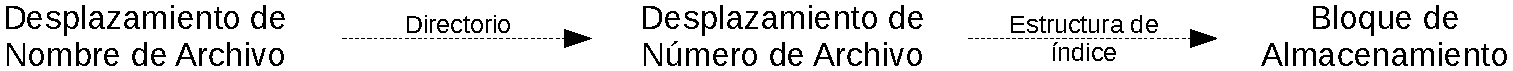
\includegraphics[scale=0.65]{img/fig1301}}
\caption{Los sistemas de archivos asignan nombres de archivos y desplazamientos de archivos a bloques de almacenamiento en dos pasos. En primer lugar, utilizan directorios para asignar nombres a números de archivo. A continuación, utilizan una estructura de índice como un árbol almacenado de forma persistente para encontrar el bloque que contiene los datos en cualquier desplazamiento específico en ese archivo.}
\label{fig1301}
\end{figure}

\textbf{Directorios y estructuras de índices}. Como se ilustra en la \textit{Fig.} \ref{fig1301}, los sistemas de archivos asignan nombres de archivos y conjuntos de archivos a bloques de almacenamiento específicos en dos pasos.

En primer lugar, utilizan directorios para asignar nombres de archivo legibles por humanos a números de archivo. Los directorios a menudo son sólo archivos especiales que contienen listas de asignaciones \textit{nombre de archivo} $\rightarrow$ \textit{número de archivo}.

En segundo lugar, una vez que un nombre de archivo se ha traducido a un número de archivo, los sistemas de archivos utilizan una estructura de índice almacenada de forma persistente para localizar los bloques del archivo. La estructura de índice puede ser cualquier estructura de datos persistente que asigna un número de archivo y un desplazamiento a un bloque de almacenamiento. A menudo, para soportar eficientemente una amplia gama de tamaños de archivo y patrones de acceso, la estructura de índice es una forma de árbol.

\textbf{Mapas de espacio libre}. Los sistemas de archivos implementan mapas de espacio libre para rastrear qué bloques de almacenamiento están libres y qué bloques están en uso a medida que los archivos crecen y se contraen. Como mínimo, el mapa de espacio libre del sistema de archivos debe permitir que éste encuentre un bloque libre cuando un archivo necesita crecer, pero debido a que la ubicación espacial es importante, la mayoría de los sistemas de archivos modernos implementan mapas de espacio libre que les permiten encontrar bloques libres cerca de una ubicación deseada. Por ejemplo, muchos sistemas de archivos implementan mapas de espacio libre como mapas de bits en almacenamiento persistente.

\textbf{Heurística de la localidad}. Los directorios y las estructuras de índices permiten a los sistemas de archivos localizar los datos de archivo y los metadatos deseados sin importar dónde se almacenen, y los mapas de espacio libre les permiten localizar el espacio libre cerca de cualquier ubicación del dispositivo de almacenamiento persistente. Estos mecanismos permiten a los sistemas de archivos emplear varias políticas para decidir dónde debe almacenarse un bloque dado de un archivo dado.

Estas políticas se materializan en \textit{heurísticas de localidad} para agrupar datos para optimizar el rendimiento. Por ejemplo, algunos sistemas de archivos agrupan los archivos de cada directorio, pero esparcen diferentes directorios a diferentes partes del dispositivo de almacenamiento. Otros desfragmentan periódicamente su almacenamiento, reescribiendo los archivos existentes para que cada archivo se almacene en bloques de almacenamiento secuencial y de modo que el dispositivo de almacenamiento tenga largas secuencias de espacio libre secuencial para que los nuevos archivos se puedan escribir secuencialmente. Y otros optimizan escrituras vs. lecturas, y escriben todos los datos secuencialmente, si un conjunto dado de escrituras contiene actualizaciones a un archivo o a muchos otros.

\section{Directorios: nombres de datos}
Como indica la \textit{Fig.} \ref{fig1301} para acceder a un archivo, el sistema de archivos traduce primero el nombre del archivo a su número. Por ejemplo, el archivo denominado {\mf /home/tom/foo.txt} puede conocerse internamente como archivo {\mf 66212871}. Los sistemas de archivos utilizan directorios para almacenar sus asignaciones de nombres legibles por humanos a números de archivos internos y organizan estos directorios de forma jerárquica para que los usuarios puedan agrupar Archivos relacionados y directorios.

\begin{figure}[tbhp]
\centerline{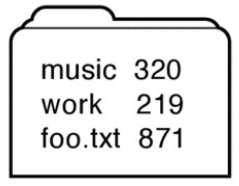
\includegraphics[scale=0.45]{img/fig1302}}
\caption{Un directorio es un archivo que contiene una colección de asignaciones (\textit{nombre de archivo} $\rightarrow$ \textit{número de archivo}).}
\label{fig1302}
\end{figure}

La implementación de directorios de una manera que proporciona mapeos jerárquicos de nombre a número resulta ser simple: se utilizan archivos para almacenar directorios. Por lo tanto, si el sistema necesita determinar el número de un archivo, sólo puede abrir el archivo de directorio apropiado y escanear a través de los pares (nombre de archivo/número de archivo) hasta encontrar el correcto.

Por ejemplo, la \textit{Fig.} \ref{fig1302} ilustra el contenido de un único archivo de directorio. Para abrir el archivo {\mf foo.txt}, el sistema de archivos analizará este archivo de directorio, encontrará la entrada {\mf foo.txt} y verá que el archivo {\mf foo.txt} tiene el número de archivo {\mf 66212871}.

\begin{figure}[tbhp]
\centerline{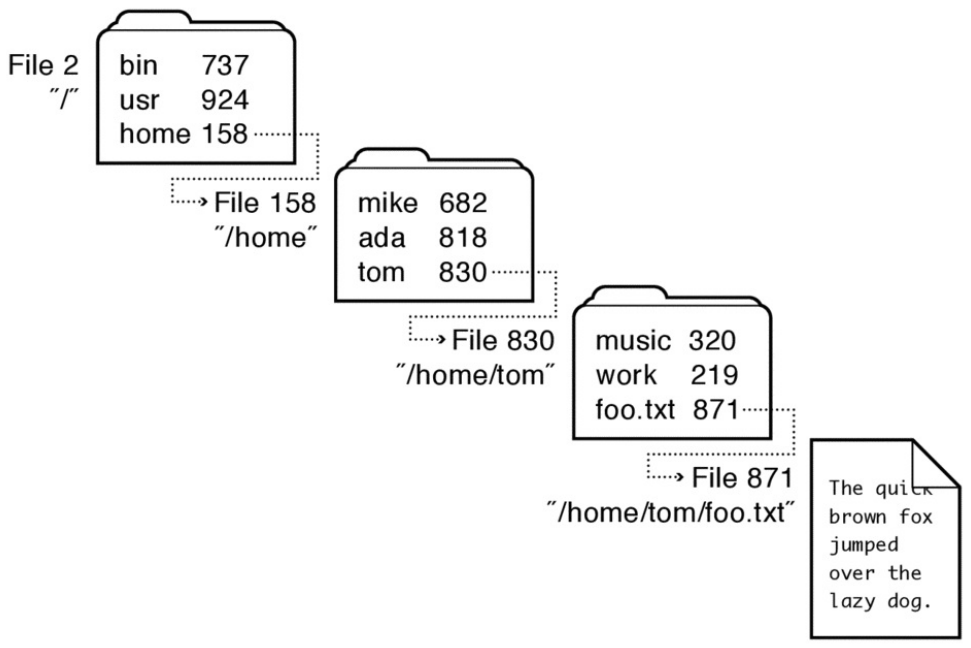
\includegraphics[scale=0.45]{img/fig1303}}
\caption{Los directorios pueden organizarse jerárquicamente al tener un directorio que contenga la asignación (\textit{nombre de archivo} $\rightarrow$ \textit{número de archivo}) para otro directorio.}
\label{fig1303}
\end{figure}

Por supuesto, si usamos archivos para almacenar el contenido de directorios como {\mf /home/tom}, todavía tenemos el problema de encontrar los archivos de directorio en sí. Como se muestra en la \textit{Fig.} \ref{fig1303}, el número de archivo del directorio {\mf /home/tom} se puede encontrar buscando el nombre {\mf tom} en el directorio {\mf /home} y el número de archivo para directorio {\mf /home} se puede buscar buscando el nombre {\mf home} en el directorio raíz {\mf /}.

Los algoritmos recursivos necesitan un caso base: no podemos descubrir el número de archivo de directorios raíz mirando en algún otro directorio. La solución es acordar el número de archivo del directorio raíz con antelación. Por ejemplo, el \textbf{Fast File System} (FFS) de Unix y muchos otros sistemas de archivos Unix y Linux usan {\mf 2} como el número de archivo predefinido para el directorio raíz de un sistema de archivos.

Por lo tanto, para leer el archivo {\mf /home/tom/foo.txt} en la \textit{Fig.} \ref{fig1303}, leemos primero el directorio raíz leyendo el archivo con la bien conocida raíz número {\mf 2}. En ese archivo, buscamos el nombre {\mf home} y encontramos que directorio {\mf /home} está almacenado en el archivo {\mf 88026158}. Leyendo el archivo {\mf 88026158} y buscando el nombre {\mf tom}, aprendemos que directorio {\mf /home/tom} está almacenado en el archivo {\mf 5268830}. Finalmente, por Leyendo archivo {\mf 5268830} y buscando el nombre {\mf foo.txt}, nos enteramos de que {\mf /home/tom/foo.txt} es el número de archivo {\mf 66212871}.

Aunque buscar el número de un archivo puede tomar varios pasos, esperamos que haya localidad (por ejemplo, cuando se accede a un archivo en un directorio, es muy probable que pronto se acceda a otros archivos del mismo directorio), por lo que esperamos que el almacenamiento en caché reduzca el número de accesos de disco necesarios para la mayoría de las búsquedas.

\textbf{API de directorios}. Los directorios utilizan una API especializada porque deben controlar el contenido de estos archivos. Por ejemplo, los sistemas de archivos deben evitar que las aplicaciones corrompan la lista de asignaciones (\textit{nombre de archivo} $\rightarrow$ \textit{número de archivo}), lo que podría impedir que el sistema operativo realice búsquedas o actualizaciones. Como otro ejemplo, el sistema de archivos debe hacer cumplir el invariante de que cada número de archivo en una entrada de directorio válida se refiere a un archivo que realmente existe.

Por lo tanto, los sistemas de archivos proporcionan llamadas especiales al sistema para modificar los archivos de directorio. Por ejemplo, en lugar de utilizar la llamada de sistema de escritura estándar para agregar una entrada de un nuevo archivo a un directorio, las aplicaciones utilizan la llamada {\mf create}. Al restringir las actualizaciones, estas llamadas garantizan que los archivos de directorio siempre pueden ser analizados por el sistema operativo. Estas llamadas también enlazan la creación o eliminación de un archivo y la entrada de directorio del archivo, de modo que las entradas de directorio siempre se refieren a archivos reales y que todos los archivos tienen al menos una entrada de directorio.

\textbf{Detalles internos de los directorios}. Muchas de las primeras implementaciones de sistemas de archivos simplemente almacenaban listas lineales de pares (nombre de archivo/número de archivo) en archivos de directorio. Por ejemplo, en la versión original del sistema de archivos ext2 de Linux, cada archivo de directorio almacenaba una lista vinculada de entradas de directorio como se ilustra en la \textit{Fig.} \ref{fig1304}.

\begin{figure}[tbhp]
\centerline{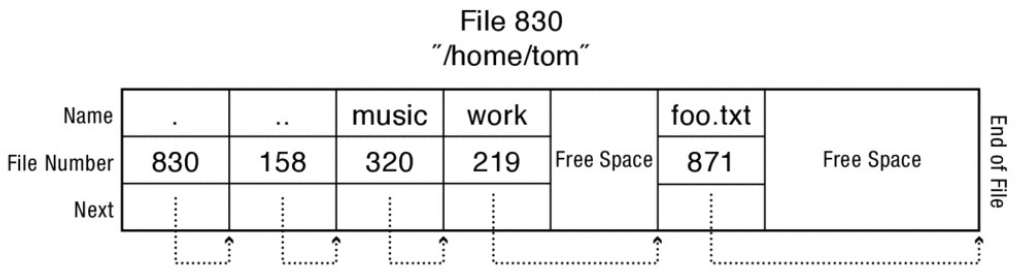
\includegraphics[scale=0.50]{img/fig1304}}
\caption{Una implementación de lista vinculada de un directorio. Este ejemplo muestra un archivo de directorio que contiene cinco entradas: {\mf music}, {\mf work} y {\mf foo.txt}, junto con {\mf .} (el directorio actual) y {\mf ..} (el directorio padre).}
\label{fig1304}
\end{figure}

Las listas simples funcionan bien cuando el número de entradas de directorio es pequeño. Una vez que un directorio tiene unos pocos miles de entradas, los directorios basados en listas simples se vuelven lentos.

Para soportar de forma eficaz directorios con muchas entradas, muchos sistemas de archivos recientes, incluyendo XFS de Linux y NTFS de Microsoft, entre otros, aumentan la lista vinculada subyacente con una estructura adicional basada en hash para acelerar las búsquedas. Estos sistemas de archivos implementan registros de directorio que mapean nombres de archivo a números de archivo y dichas asignaciones se almacenan en un \textbf{árbol B+} indexado por el hash del nombre de cada archivo. Para encontrar el número de archivo de un nombre de archivo dado, el sistema de archivos calcula primero un hash del nombre. A continuación, utiliza ese hash como clave para buscar la entrada del directorio en el árbol: comenzando en la raíz del árbol B+ en un desplazamiento bien conocido en el archivo y procediendo a través de los nodos internos hacia los nodos hoja del árbol. En cada nivel, un nodo contiene una matriz de pares (clave de hash/desplazamiento de archivo) que representan cada uno un puntero al nodo secundario que contiene entradas con claves más pequeñas que la clave de hash pero mayores que la clave de hash de la entrada anterior. El sistema de archivos busca en el nodo la primera entrada con un valor de clave de hash que excede la clave de destino y, a continuación, sigue el puntero de desplazamiento de archivo correspondiente al nodo secundario correcto. El puntero de desplazamiento de archivo en el registro en los nodos hoja apunta a la entrada de directorio de destino.

\textbf{Hard y soft links}. Muchos sistemas de archivos permiten que un archivo dado tenga varios nombres. Los \textbf{hard links} o enlaces duros son varias entradas de directorio de archivos que asignan nombres de ruta diferentes al mismo número de archivo. Debido a que un número de archivo puede aparecer en varios directorios, los sistemas de archivos deben asegurarse de que un archivo sólo se elimina cuando se ha eliminado el último hard link.

Para implementar correctamente la recolección de basura, los sistemas de archivos usan recuentos de referencia almacenando con cada archivo el número de enlaces duros a él. Cuando se crea un archivo, tiene un recuento de referencia de uno, y cada enlace duro adicional hecho al archivo incrementa su recuento de referencias. Por el contrario, cada llamada a desvincular disminuye el recuento de referencia del archivo y cuando el recuento de referencia cae a cero, el archivo subyacente se elimina y sus recursos se marcan como libres.

Por otra parte, en lugar de asignar un nombre de archivo a un número de archivo, los \textbf{soft links} o enlaces simbólicos son entradas de directorio que asignan un nombre a otro nombre.

\begin{figure}[tbhp]
\centerline{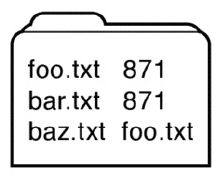
\includegraphics[scale=0.50]{img/fig1305}}
\caption{En este directorio, los hard links {\mf foo.txt} y {\mf bar.txt} y el soft link {\mf baz.txt} se refieren todos al mismo archivo.}
\label{fig1305}
\end{figure}

Por ejemplo, \textit{Fig.} \ref{fig1305} muestra un directorio que contiene tres nombres y todos se refieren al mismo archivo. Las entradas {\mf foo.txt} y {\mf bar.txt} son enlaces duros con el mismo archivo (número 66212871); {\mf baz.txt} es un enlace suave a {\mf foo.txt}. Debe notarse que si eliminamos la entrada {\mf foo.txt} de este directorio utilizando la llamada de sistema de desvinculación, el archivo todavía se puede abrir con el nombre {\mf bar.txt}, pero si intentamos abrirlo con el nombre {\mf baz.txt}, el intento fallará.


\section{Archivos: Búsqueda de datos}
Una vez que un sistema de archivos ha traducido un nombre de archivo a un número de archivo utilizando un directorio, el sistema de archivos debe ser capaz de encontrar los bloques que pertenecen a ese archivo. Además de este requisito funcional, las implementaciones de archivos suelen tener como objetivo otros cinco objetivos:
\begin{itemize}
\item Soportar la colocación secuencial de datos para maximizar el acceso secuencial a archivos.
\item Proporcionar acceso aleatorio eficiente a cualquier bloque de archivos.
\item Limitar las cargas de sistema (\textit{overheads}) para ser eficiente para archivos pequeños.
\item Ser escalable para admitir archivos grandes.
\item Proporcionar un lugar para almacenar metadatos por archivo, como el número de referencia del archivo, el propietario, la lista de control de acceso, el tamaño y el tiempo de acceso.
\end{itemize}

\subsection{FAT: Lista enlazada}
El sistema de archivos \textbf{FAT -- File Allocation Table} de Microsoft (Tabla de Asignación de Archivos) se implementó por primera vez a finales de los años setenta y era el sistema de archivos principal para MS-DOS y las primeras versiones de Microsoft Windows. El sistema de archivos FAT se ha mejorado de muchas maneras a lo largo de los años. La versión FAT-32 soporta volúmenes con hasta $2^{28}$ bloques y archivos con hasta $2^{32} - 1$ bytes.

\textbf{Estructuras de índices}. El sistema de archivos FAT recibe el nombre de su tabla de asignación de archivos, una matriz de entradas de 32 bits en un área reservada del volumen. Cada archivo del sistema corresponde a una lista vinculada de entradas FAT, con cada entrada FAT conteniendo un puntero a la siguiente entrada FAT del archivo (o un valor especial de ``fin de archivo''). La FAT tiene una entrada para cada bloque en el volumen y los bloques del archivo son los bloques que corresponden a las entradas FAT del archivo: si la entrada FAT i es la entrada i-ésima de un archivo, entonces el bloque de almacenamiento i es el i-ésimo bloque de datos del archivo.

\begin{figure}[tbhp]
\centerline{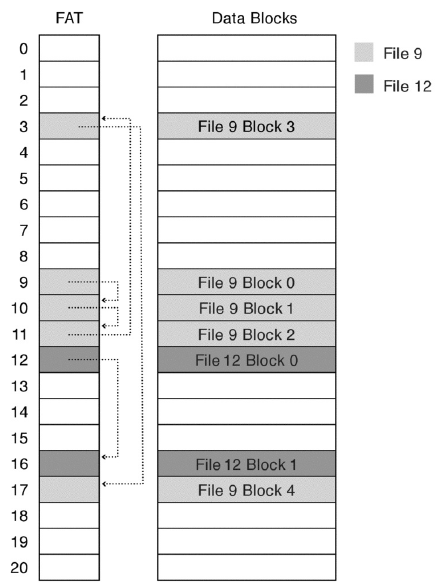
\includegraphics[scale=0.65]{img/fig1306}}
\caption{Un sistema de archivos FAT con un archivo de 5 bloques y un archivo de 2 bloques.}
\label{fig1306}
\end{figure}

La \textit{Fig.} \ref{fig1306} ilustra un sistema de archivos FAT con dos archivos. La primera comienza en el bloque {\mf 9} y contiene cinco bloques. El segundo comienza en el bloque {\mf 12} y contiene dos bloques.

Los directorios asignan nombres de archivo a números de archivo y, en el sistema de archivos FAT, el número de un archivo es el índice de la primera entrada del archivo en el FAT. Por lo tanto, dado el número de un archivo, podemos encontrar la primera entrada FAT y el bloque de un archivo, y dada la primera entrada FAT, podemos encontrar el resto de las entradas y bloques FAT del archivo.

\textbf{Seguimiento de espacio libre}. FAT también se utiliza para el seguimiento de espacio libre. Si el bloque de datos i está libre, entonces FAT[i] contiene un 0. Así, el sistema de archivos puede encontrar un bloque libre escaneando a través de la FAT para encontrar una entrada cero.

\textbf{Heurística de localidad}. Diferentes implementaciones de FAT pueden utilizar diferentes estrategias de asignación, pero las estrategias de asignación de implementaciones de FAT son generalmente simples. Por ejemplo, algunas implementaciones utilizan un algoritmo de ajuste siguiente (\textit{next fit}) que escanea secuencialmente a través de la FAT a partir de la última entrada asignada y que devuelve la siguiente entrada libre encontrada.

Estrategias de asignación simples como ésta pueden fragmentar un archivo, extendiendo los bloques del archivo a través del volumen en lugar de lograr el diseño secuencial deseado. Para mejorar el rendimiento, los usuarios pueden ejecutar una herramienta de \textbf{desfragmentación} que lee archivos de sus ubicaciones existentes y los vuelve a escribir a nuevas ubicaciones con una mejor localidad espacial. El desfragmentador FAT en Windows XP, por ejemplo, intenta copiar los bloques de cada archivo que se extiende a través de múltiples extensiones a una extensión secuencial única que contiene todos los bloques de un archivo.

\textbf{Usos y limitaciones}. El sistema de archivos FAT se utiliza ampliamente porque es simple y compatible con muchos sistemas operativos. Por ejemplo, muchas dispositivos de almacenamiento flash  USB y tarjetas de almacenamiento de cámaras utilizan el sistema de archivos FAT, permitiendo que sean leídos y escritos por casi cualquier computadora que ejecute casi cualquier sistema operativo moderno.

El sistema de archivos FAT, sin embargo, está limitado de muchas maneras. Por ejemplo,
\begin{itemize}
\item \textbf{Pobre empleo de la localidad}. Las implementaciones de FAT suelen utilizar estrategias de asignación sencillas, como el ajuste siguiente ya descrito. Estos pueden conducir a archivos mal fragmentados.
\item \textbf{Acceso aleatorio deficiente}. El acceso aleatorio dentro de un archivo requiere el desplazamiento secuencial de las entradas FAT del archivo hasta que se alcance el bloque deseado.
\item \textbf{Metadatos limitados de archivos y control de acceso}. Los metadatos de cada archivo incluyen información como el nombre, el tamaño y el tiempo de creación del archivo, pero no incluyen información de control de acceso, como el propietario del archivo o el ID de grupo, para que cualquier usuario pueda leer o escribir cualquier archivo almacenado en un sistema de archivos FAT.
\item \textbf{No hay soporte para enlaces duros}. FAT representa cada archivo como una lista vinculada de entradas de 32 bits en la tabla de asignación de archivos. Esta representación no incluye espacio para otros metadatos de archivo. En su lugar, los metadatos de archivo son almacenados como entradas de directorio con el nombre del archivo. Este enfoque exige que cada archivo se acceda a través de una entrada de directorio exactamente, descartando múltiples enlaces duros a un archivo.
\item \textbf{Limitaciones en volumen y tamaño de archivo}. Las entradas de tabla FAT son de 32 bits, pero los cuatro bits superiores se encuentran reservados. Así, un volumen FAT puede tener como máximo $2^{28}$ bloques. Con bloques de 4 KB, el tamaño máximo de volumen está limitado (por ejemplo, $2^{28} \frac{\text{bloques}}{\text{volumen}} \times 2^{12}\frac{\text{bytes}}{\text{bloque}} = 2^{40}\frac{\text{bytes}}{\text{volumen}} =$ 1 TB). Se admiten bloques de hasta 256 KB, pero se corre el riesgo de perder grandes cantidades de espacio en disco debido a la fragmentación interna. Del mismo modo, los tamaños de archivo se codifican en 32 bits, por lo que ningún archivo puede ser mayor que $2^{32} - 1$ bytes (poco menos de 4 GB).
\item \textbf{Falta de soporte para técnicas modernas de confiabilidad}. FAT no admite las técnicas de actualización transaccional que
los sistemas de archivos modernos utilizan para evitar la corrupción de las estructuras de datos críticos si el equipo se bloquea mientras se escribe en el almacenamiento.
\end{itemize}




%------------------------------------------------------------------------------------------------------------------------------------------
%	BIBLIOGRAFÍA
%------------------------------------------------------------------------------------------------------------------------------------------
\nocite{*}
\bibliographystyle{resumen}
\bibliography{resumen}


\end{document}